
\documentclass[12pt]{article}

\usepackage{graphicx}
\graphicspath{ {./images/} }

\usepackage{epsfig}
\usepackage{amsmath,amsthm}
\usepackage{listings}


\newtheorem{lemma}{Lemma}
\newtheorem{theorem}{Theorem}


\usepackage{titlesec}
\titleformat{\section}
{\normalfont\Large\bfseries}{Question~\thesection:}{1em}{}

\newlength{\toppush}
\setlength{\toppush}{2\headheight}
\addtolength{\toppush}{\headsep}


\def\subjnum{Comp 160}
\def\subjname{Algorithms}


\def\doheading#1#2#3{\vfill\eject\vspace*{-\toppush}%
  \vbox{\hbox to\textwidth{{\bf} \subjnum: \subjname \hfil Erli Cai}%
    \hbox to\textwidth{{\bf} Tufts University, Fall 2020 \hfil#3\strut}%
    \hrule}}


\newcommand{\htitle}[1]{\vspace*{1.25ex plus 1ex minus 0ex}%
\begin{center}
{\large\bf #1}
\end{center}} 



\begin{document}
\doheading{2}{title}{Homework 04}
\setlength\parindent{0pt}

\section{}
(a) \\
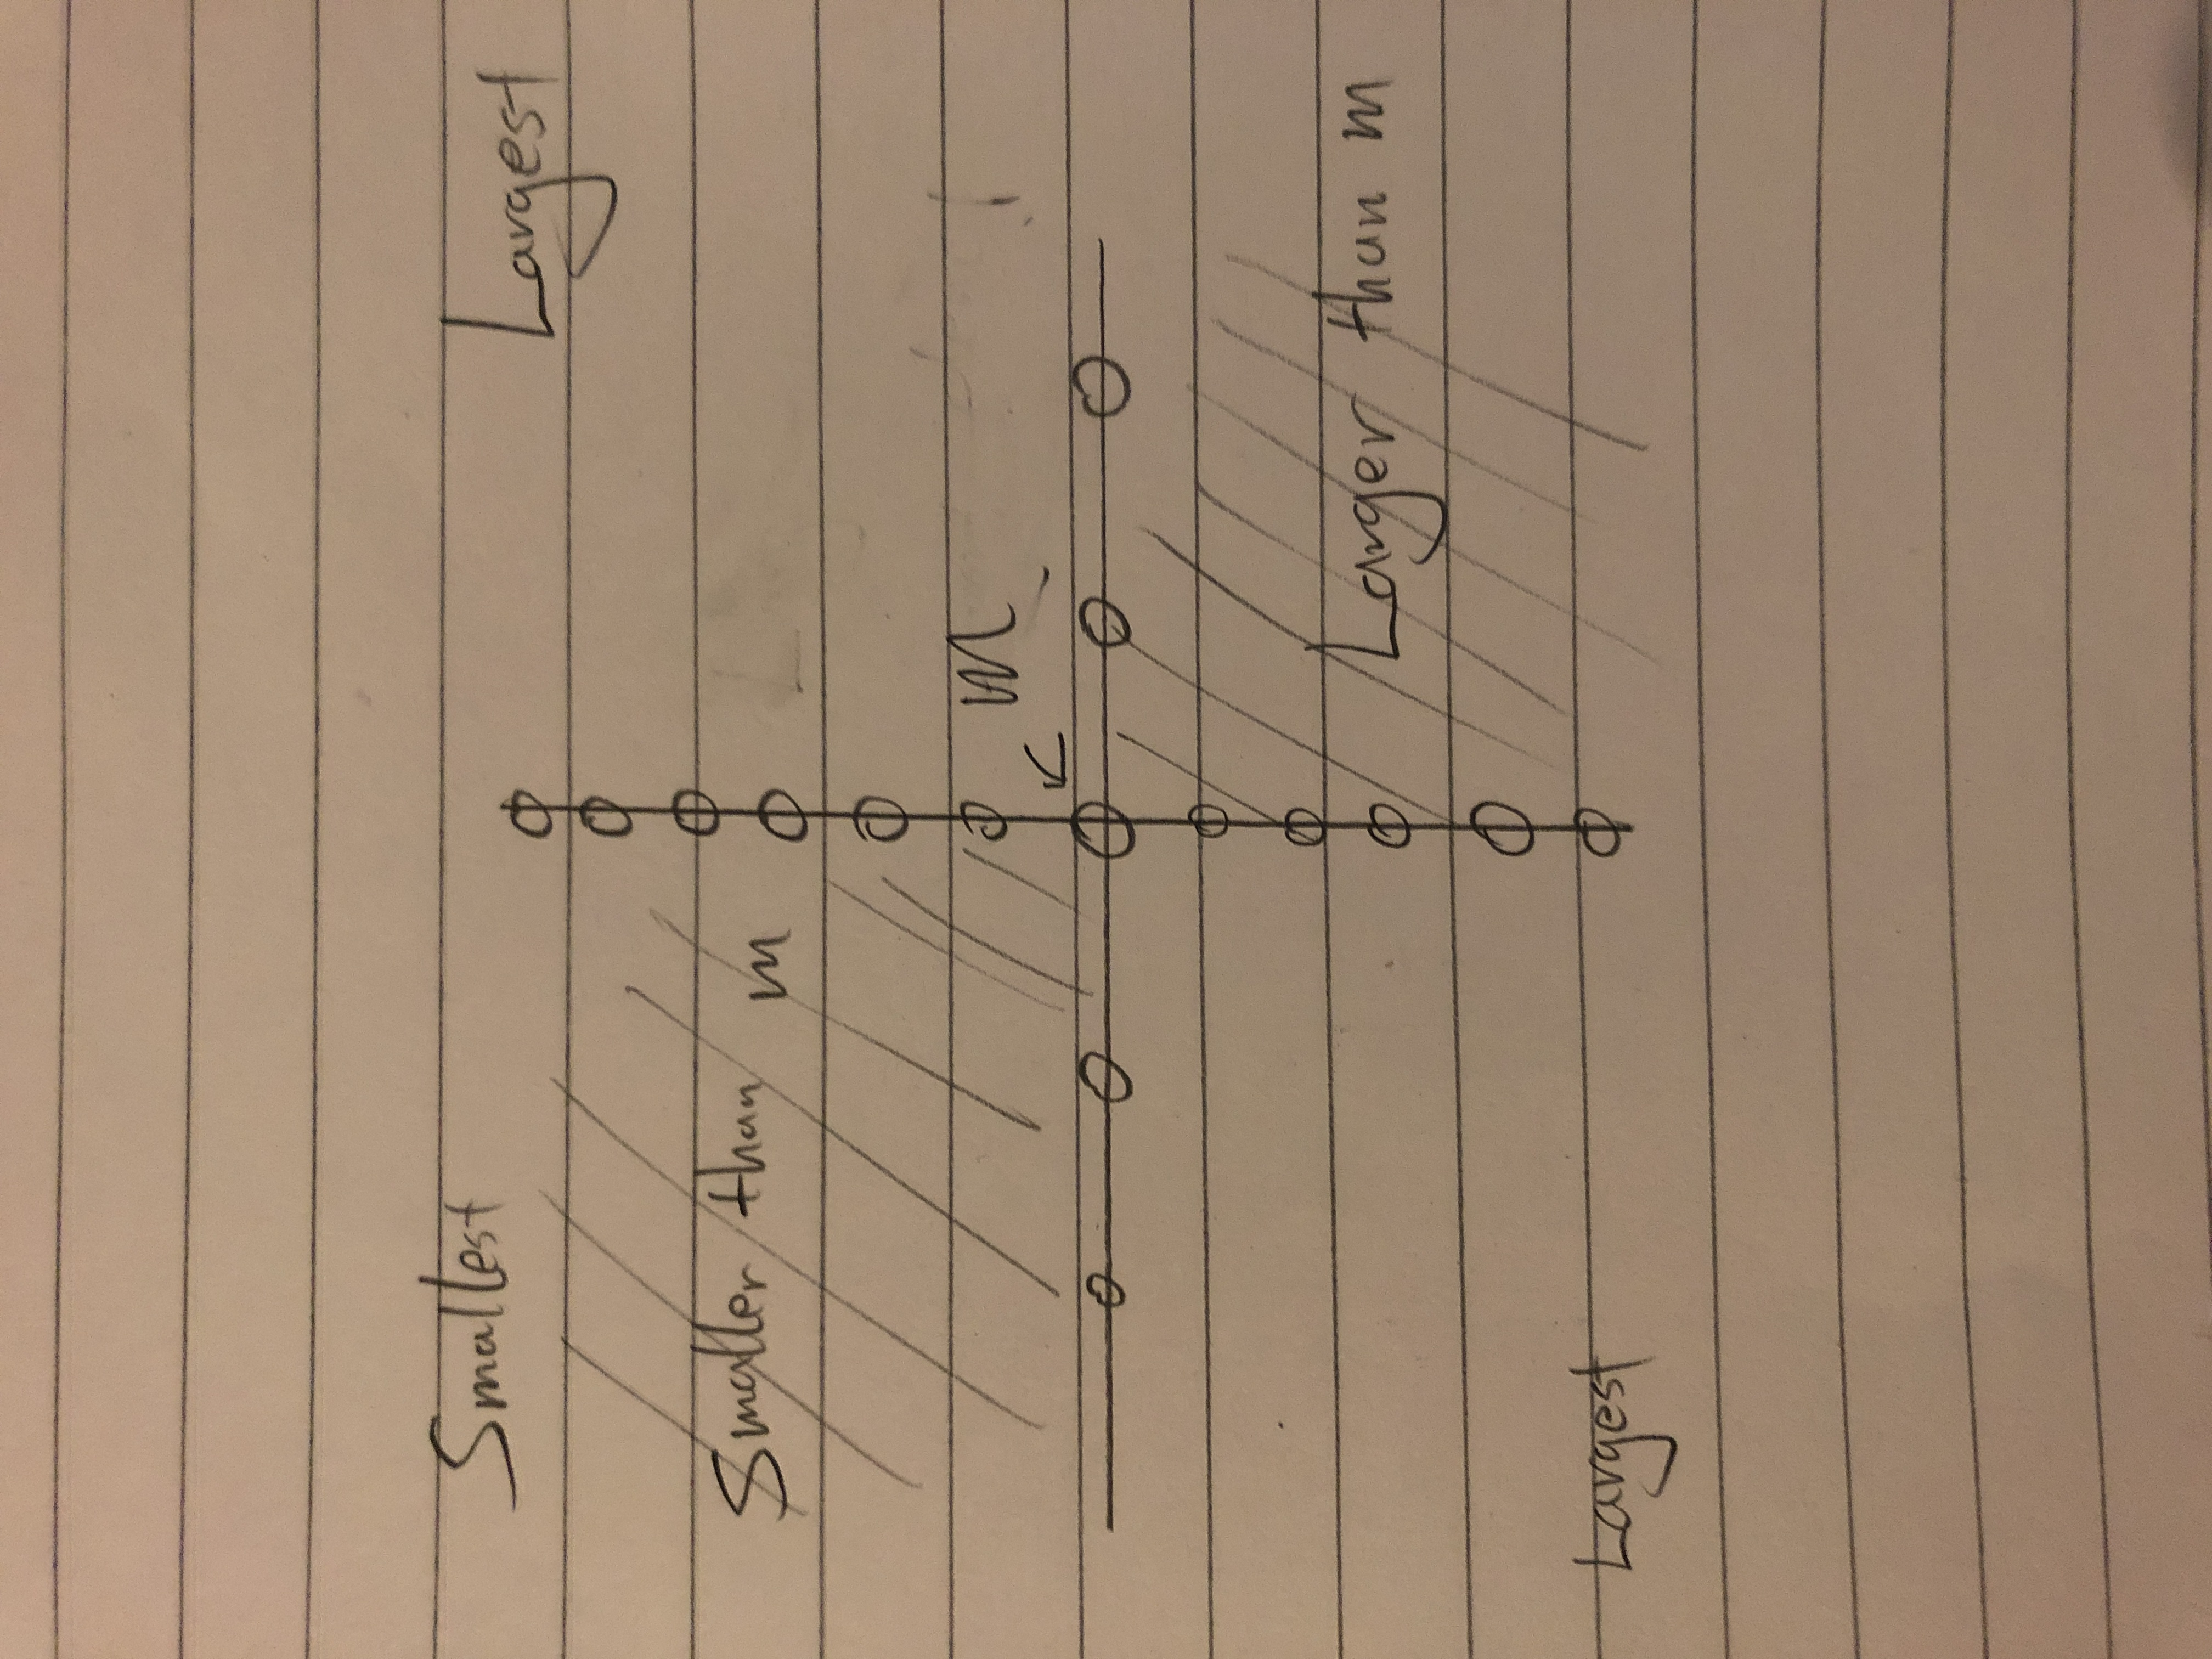
\includegraphics[scale = 0.05, angle = 270]{1.JPG}

We can see from the graph that a quarter of the elements are smaller than m and a quarter of the elements are larger than m. \\
Therefore, $ \frac{n}{4} \le i \le \frac{3n}{4}$\\

(b) 
Let T(n) be the time needed with QuickSort algorithm on problem of size n.\\
Step 1: there are n/5 groups and finding median of each takes O(1) time, so Step 1 takes O(n) time\\
Step 2: We can apply selection algorithm to find the median, so it takes linear, O(n), runtime.\\
Step 3: Partition takes linear runtime, so O(n) time\\
Step 4: we have 2 subproblems of size i-1 and size n-i+1, so step 4 takes T(i-1) + T(n-i-1) time\\

If we let $X_j = 1$ when i = j. \\
Then $T(n) = \Sigma_{j=\frac{n}{4}}^{j = \frac{3n}{4}} X_j \times(T(i-1) + T(n-i-1)) + O(n)$\\
$E(T(n)) = \Sigma_{j=\frac{n}{4}}^{j = \frac{3n}{4}} \frac{2}{n} \times(T(i-1) + T(n-i-1)) + O(n)$\\

(c) 
The runtime should be $\theta(n\log n)$

\begin{flalign*}
E(T(n)) &= \Sigma_{j=\frac{n}{4}}^{j = \frac{3n}{4}} \frac{2}{n} \times(T(i-1) + T(n-i-1)) + O(n)\\
&=  \Sigma_{j=\frac{n}{4}}^{j = \frac{3n}{4}} \frac{2}{n} \times[T(i-1) + T(n-i-1) + O(n)]
\end{flalign*}

we see that average expected runtime is averaged over n/2 cases, each have runtime $T(i-1) + T(n-i-1) + O(n)$ for $\frac{n}{4}\le i\le \frac{3n}{4}$ \\

If we solve for $ S(n) = S(i-1)+ S(n-i-1) + O(n)$ ($\frac{n}{4}\le i\le \frac{3n}{4}$),\\
 we will get $S(n) = \theta(n\log n)$

And since we are averaged over n/2 cases of $ \theta(n\log n)$ rumtime, the averaged runtime will be $ \theta(n\log n)$

\pagebreak


\section{}
(a) After partitioning and before recursing, RANDSELECT algorithm need to compare the position getting from partitioning and target position. And then choose a subproblem to solve. This step will only cost O(1) runtime since only 1 comparison is needed\\


(b) QUICKSORT need to recurse on both subproblems while RANDSELECT only need to recurse on one subproblem.\\

(c) 
Let $X_j = 1 $ if we get position j from partitioning, then\\
QUICKSORT:  $E(Q(n)) =\theta(n) + \frac{1}{n}\Sigma_j E(Q(j-1) + Q(N-j) )$\\
RANDSELECT: $E(R(n)) =\theta(n) + \frac{1}{n}\Sigma_j E(\max\{R(j-1) + R(N-j)\} )$\\

main difference between the two formulas: RANDSELECT only recur on the larger one between R(j-1) and R(n-j)\\

(d) 
Guess : $E(Q(n)) \le a\cdot n$ 
\begin{flalign*}
 E(Q(n)) &=\theta(n) + \frac{1}{n}\Sigma_{j=1}^{j=n} E(Q(j-1) + Q(n-j) ) &\\
 & \le bn + \frac{1}{n}\Sigma_{j=1}^{j=n} (a\cdot (j-1) + a\cdot Q(n-j)) \\
 & \le bn +\frac{a}{n} (n*(n-1))\\
 & \le (a+b)n - a
\end{flalign*}

No matter how we choose a, $(a+b)n -a \ge a\cdot n$ at some large n.
So our guess is false.



\pagebreak
\section{}
(a) 
Prune and incinerate :$P(n) = P(n-1) + 1$\\
After each cut, the picture is smaller by 1 unit \\
Guess $P(n) = \theta(n)$ , then $ an < P(n) < bn$ for some a,b\\
Base case: $ a < P(2) = 1 < b $\\
Induction hypothesis: $ an \le P(n) \le bn$ for all $n \ le k$\\
Induction Step: $  a(k+1)= ak+a\le P(k+1) = P(k) +1 \le bk +b = b(k+1)$\\
In conclusion, $P(n) =  \theta(n)$\\

Divide and divide again : $D(n) = 2D(n/2) + 1$\\
After each cut, we have two pieces of picture of half the size\\
Using master method, we have $n^{\log_ba} = n ^{\log_22} = n$ and f(n) = 1 = O(n),\\
thus $D(n) = \theta(n)$\\ 


Stack them up $S(n) = S(n/2) + 1$\\
After each cut, the picture in stack have half the size\\
From the recursion tree below, we see that the height of the tree is log(n).\\
Thus, the runtime will be $O(logn \cdot 1) = O(logn)$ \\
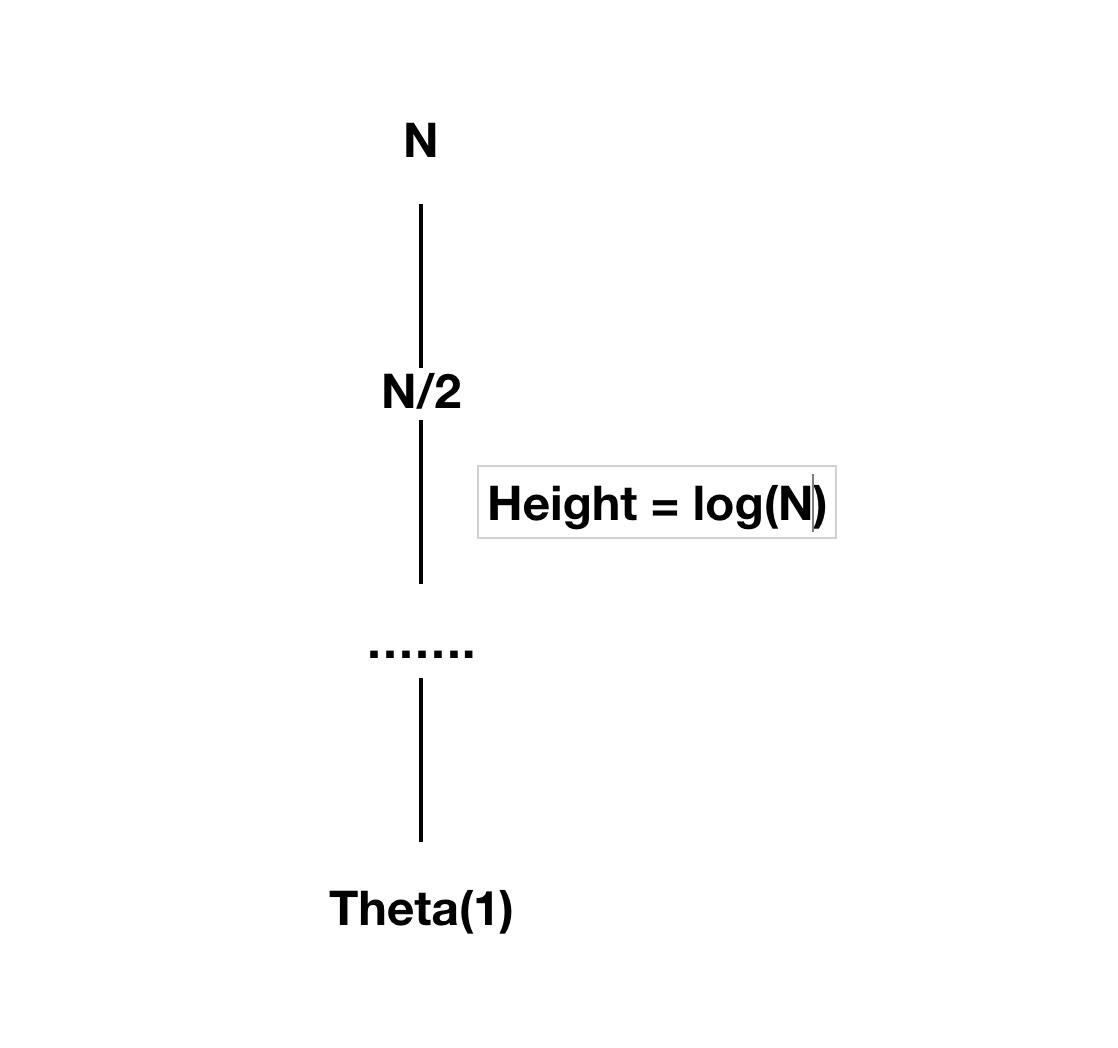
\includegraphics[scale = 0.3]{2}
\\

(b) Stack them up is the best strategy since it has the smallest asymptotic runtime.
Both Prune and incinerate and Divide and divide again has linear runtime, so they are both worst strategy.



\end{document}


